\documentclass{standalone}
\usepackage{tikz}

\begin{document}
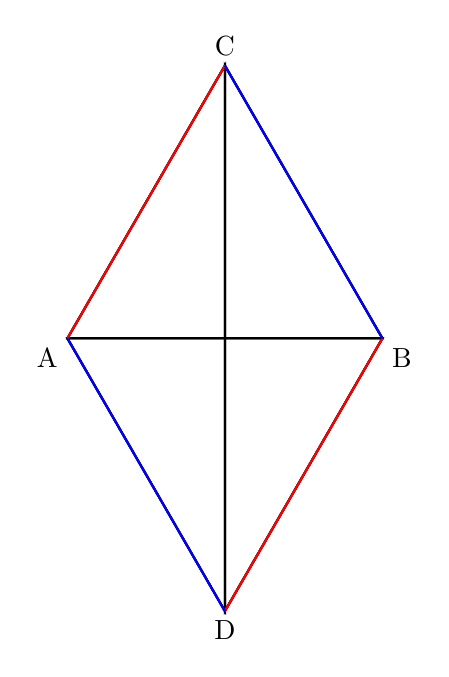
\begin{tikzpicture}[scale=2]

% Define the coordinates of the vertices
\coordinate (A) at (-1, 0);
\coordinate (B) at (1, 0);
\coordinate (C) at (0, 1.732);
\coordinate (D) at (0, -1.732);

% Draw the edges of the tetrahedron
\draw[thick] (A) -- (B) -- (C) -- cycle;
\draw[thick] (A) -- (B) -- (D) -- cycle;
\draw[thick] (A) -- (C) -- (D) -- cycle;
\draw[thick] (B) -- (C) -- (D) -- cycle;

% Draw the red lines
\draw[red, thick] (A) -- (C);
\draw[red, thick] (B) -- (D);

% Draw the blue lines
\draw[blue, thick] (A) -- (D);
\draw[blue, thick] (B) -- (C);

% Label the vertices
\node at (A) [below left] {A};
\node at (B) [below right] {B};
\node at (C) [above] {C};
\node at (D) [below] {D};

\end{tikzpicture}
\end{document}